\IEEEraisesectionheading{\section{Introduction}\label{sec:introduction}}
\label{sec:intro}


%1. What is challenge response authentication, how does it work? What’s the typical flow?
%2 What are the advantages of challenge response authentication compared with other authentication scheme?
%3. What does the traditional challenge response authentication missing?  For instance, if I got my friend’s exxon mobile easy pay, I can get gasoline with his card.  This cannot prevent insider attacks. 

%For instance, only those guards who have passed background check can be authorized to walk throughout the building. Verifying their identities is important.  Therefore, we introduce a biometric-based challenge response scheme.  We don’t use fingerprint because of the privacy concern…….

%4. Why we use motion?  Because depth sensors becomes pervasive, and it is a behavor based biometrics
%5. Why it’s challenging, because we have to ask users to write different content yet still authenticate it correctly. 
%6. What’s our basic idea? model the writing style instead of what he/she writes…..


User authentication is one of the most important yet challenging tasks in computer security~\cite{Uell:CCS13,Monrose:CCS99,Zheng:CCS11,Ahmed:TPDS07,Ari:CCS13}. The difficulty stems from the insecure communication, where eavesdropping, man-in-the-middle attacks, and replay attacks are all made possible. Challenge-response (CR) authentication can effectively cope with these attacks: typically, during a CR authentication, one party (e.g., a server) sends a random challenge. To be authenticated, the other party (e.g., a user) has to send back a valid response, which is usually the hash of the challenge and the secret shared by the two parties beforehand. Because the challenge is randomly selected and it is difficult to extract the password from the response,  CR authentication is considered secure over insecure communication channels.  However, such a challenge response method authenticates is based on \textit{what you know} instead of \textit{who you are}. Anyone knowing the shared secret can pass the authentication. Such authentication cannot prevent insider attacks, which are serious threats to systems with strict security requirements. For instance, enterprise or government may only allow the security guards who have passed extensive background checks to patrol their buildings. Letting their friends or colleagues without background checks substitute them is not allowed and can lead to an insider attack. To address it, we study biometric-based challenge-response schemes to authenticate based on \textit{who you are}. \jing{Compared with authentication using biometrics, adding the procedure of challenge-response will introduce an extra amount of time to verify the response. Nevertheless, we believe the challenge-response procedure can reduce the possibility of replay attacks.}


\begin{figure}[t]
\vspace{-5mm}
\centering
{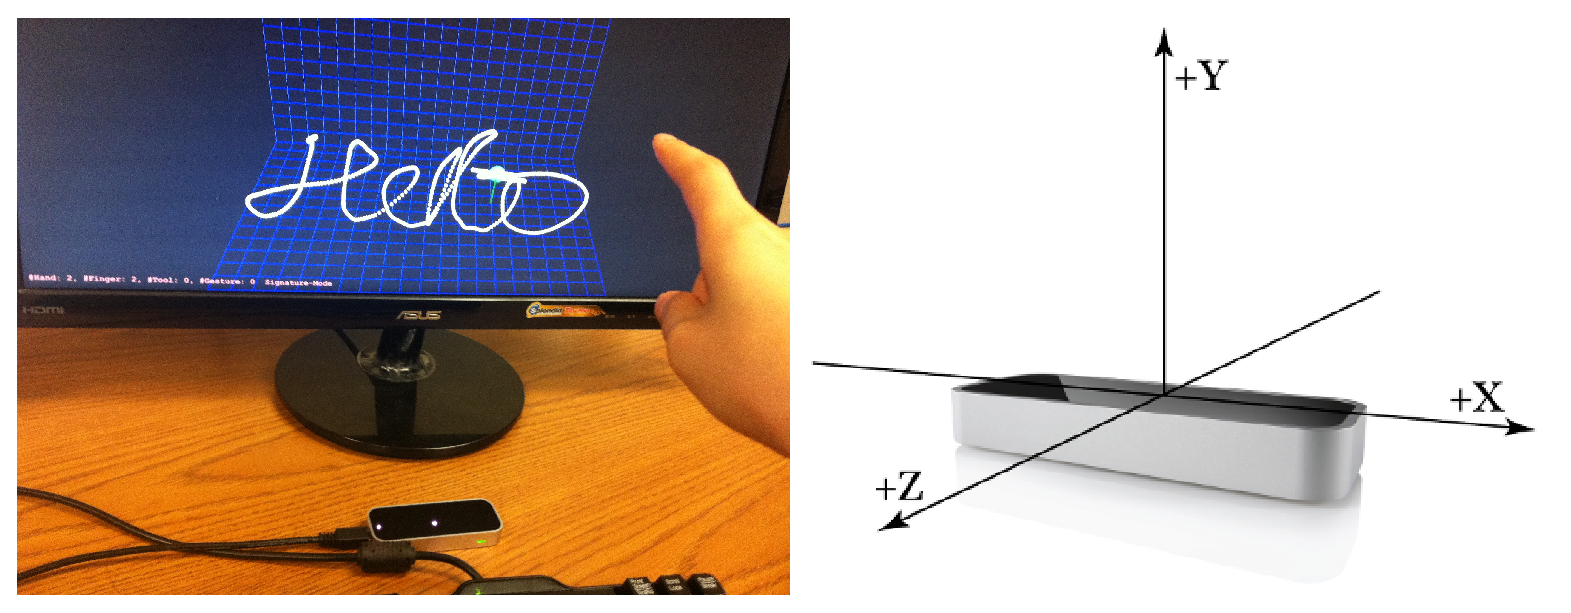
\includegraphics[width=.9\columnwidth]{./Graphic/SystemFlow/leap_motion_system.eps}} %LP.pdf
\caption{{An illustration of using a Leap Motion controller to acquire a user's handwriting in the 3D space for content independent CR authentication.}\vspace{-5mm}}\label{fig:leap}
\end{figure}





Both physical and behavioral biometrics can be used to identify who you are. Considering that physical biometrics are not privacy-friendly and are limited in numbers, we focus on designing a behavioral-biometric-based CR authentication system.
%\jing{We envision to design a motion-based authentication system with the following features. First, it works in a contactless manner, which has the benefit to elliminate hygiene concerns and is resilient to smudge attacks~\cite{Aviv:woot10}, i.e., finger smudges (due to oily residues) on a touch screen can reveal passwords. Second, it can be used as a complementary method when traditional biometrics-based authentication is inapplicable. For instance, fingerprints are inapplicable in several scenarios, e.g., fingerprints are unsuitable to users with dirty, greasy, or worn-out fingerprints due to their professions (e.g., miners). Third, it should be applicable to the public scenarios and thus should be resistant to shoulder surfing (i.e., observing) attacks, and acoustic environmental noises. } 
\jing{
We propose to use in-air handwriting style as a new biometrics for authentication. We use a depth motion sensor, Leap Motion controller~\cite{LeapOnline1} to record in-air fingertip writings as shown in Figure~\ref{fig:leap}. \jingap{Handwriting samples}, in the form of scanned images or recorded by tablet, have been used as signature verification or writer identification for authorization or forensics purpose~\cite{Schomaker:2008}. Compared to writings on tablet, the in-air writings introduce a larger amount of variability which we believe contain a richer set of biometric yet introduce extra intra-variance for multiple trial of writings from the same writer, and thus impose challenges for authentication. 

Despite of the challenge, we choose in-air handwriting because it has the following advantages. First, it does not require physical contact to any device. Thus, it elliminates hygiene concerns and is resilient to smudge attacks~\cite{Aviv:woot10}, i.e., finger smudges (due to oily residues) on a touch screen can reveal passwords.  Second, handwriting style is essentially a behavioral biometrics and thus has limited privacy issue. Third, given the rich combination of letters and numbers, the continuously written words are challenging to be synthesized because we believe that imitating arbitrary handwritings in the three dimensional (3D)-space is ambitious, making it resistant to shoulder surfing.}  Last but not least, it can be used as a complementary method when traditional biometrics-based authentication is inapplicable. For instance, fingerprints are inapplicable in several scenarios, e.g., fingerprints are unsuitable to users with dirty, greasy, or worn-out fingerprints due to their professions (e.g., miners). 


We call the proposed behavioral-biometric-based CR authentication system as \CiT. Specifically, we use data extracted from finger movements when a user writes in the air.
The \CiT system works as follows. To authenticate a user, \CiT randomly prompts a string (e.g., a few words) on the screen as a challenge, and the user has to write the string in the air as a response. Then the system performs two steps. First, determine whether the content of the handwriting is the same as the challenge. Second, verify if the handwriting is created by the user. Since  handwriting recognition can utilize existing technology~\cite{Tappert1990} and recent study shows that Leap Motion has the potential for handwriting recognition application~\cite{Vikram_handwritingleap, ICDAR15:OnlineHandwriting}, this paper focuses on the second step --- user verification based on the in-air handwriting. 


\begin{figure}[!t]
\centering
\begin{tabular}{cccccc}
\hline 
\vspace{2mm}
User-1
&
{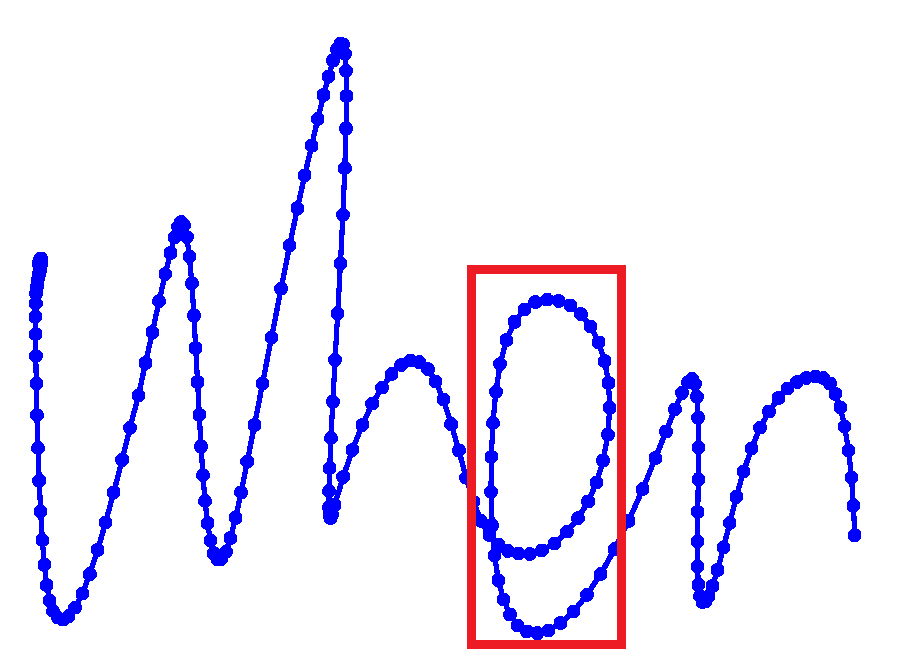
\includegraphics[width=0.09\columnwidth]{./Graphic/words_jing/1001_pdfCopy.eps}}
%&
%{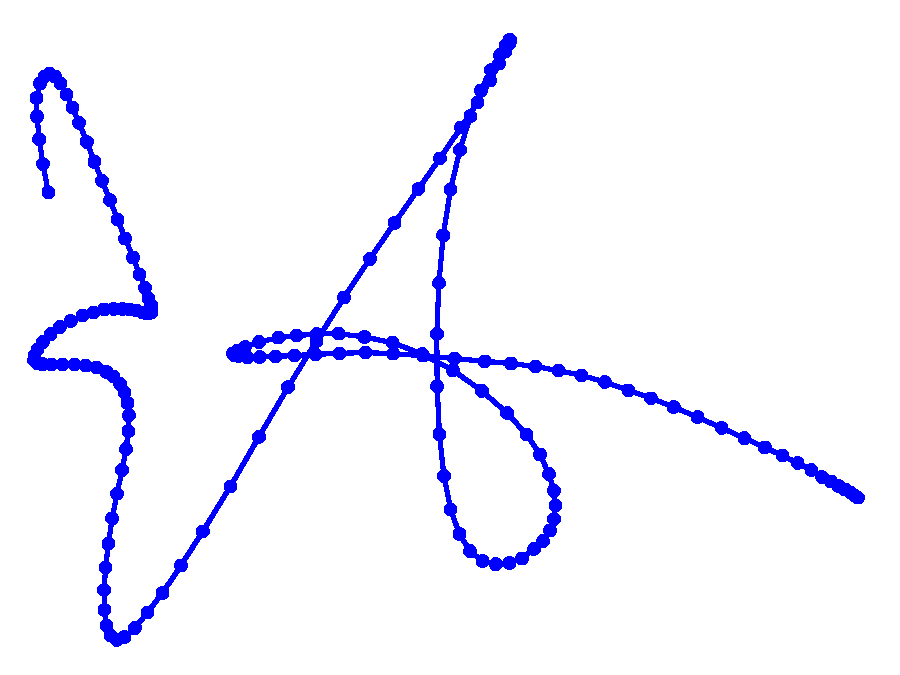
\includegraphics[width=0.09\columnwidth]{./Graphic/words_jing/1002_pdf.eps}}
& 
{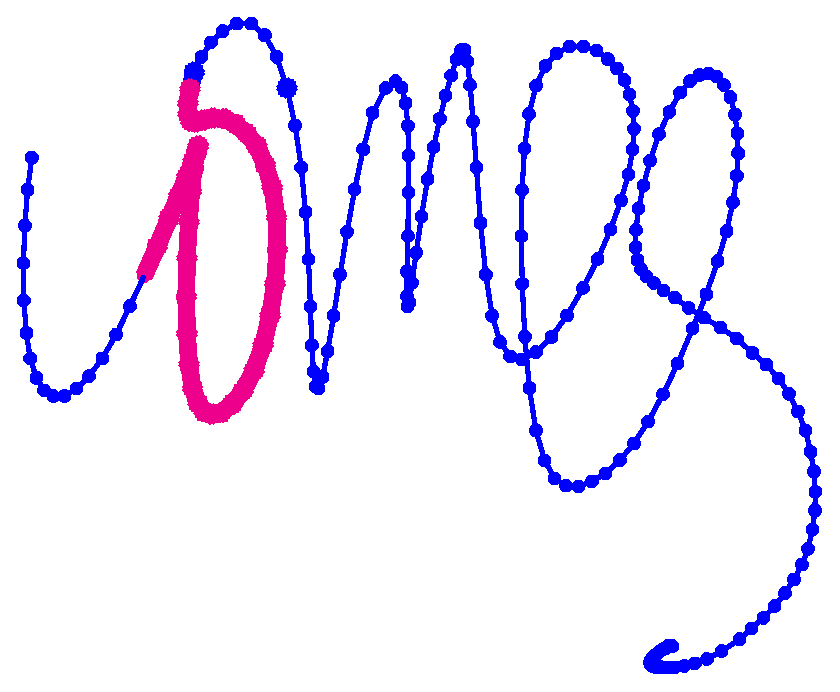
\includegraphics[width=0.09\columnwidth]{./Graphic/words_jing/1003_pdfCopy.eps}}
%& 
%{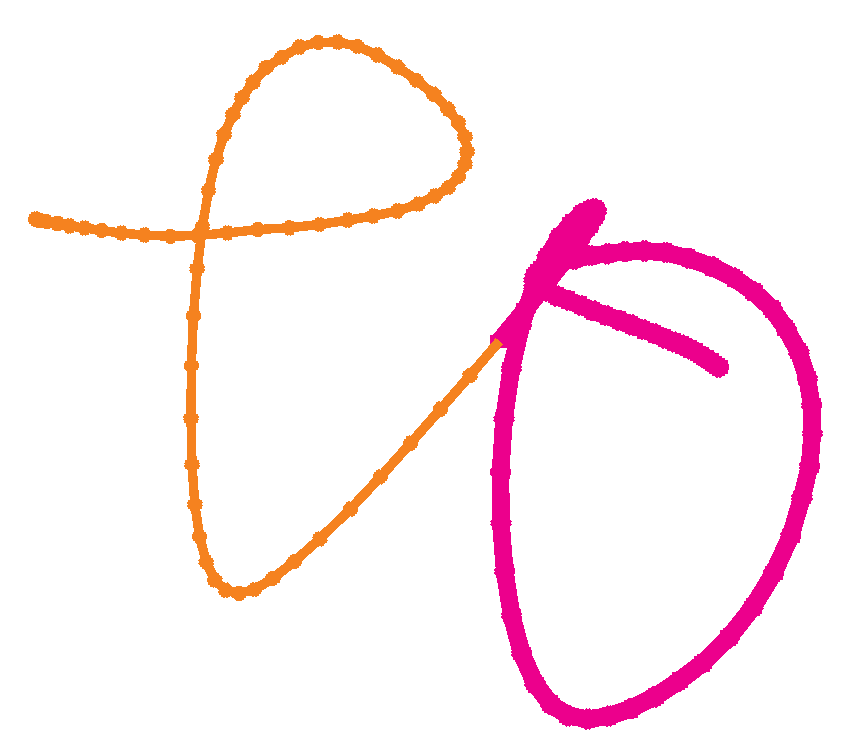
\includegraphics[width=0.09\columnwidth]{./Graphic/words_jing/1004_pdfCopy.eps}}
%& 
%{
\includegraphics[width=0.19\columnwidth]{./Graphic/words_jing/1005_pdf.eps}}
%& 
%{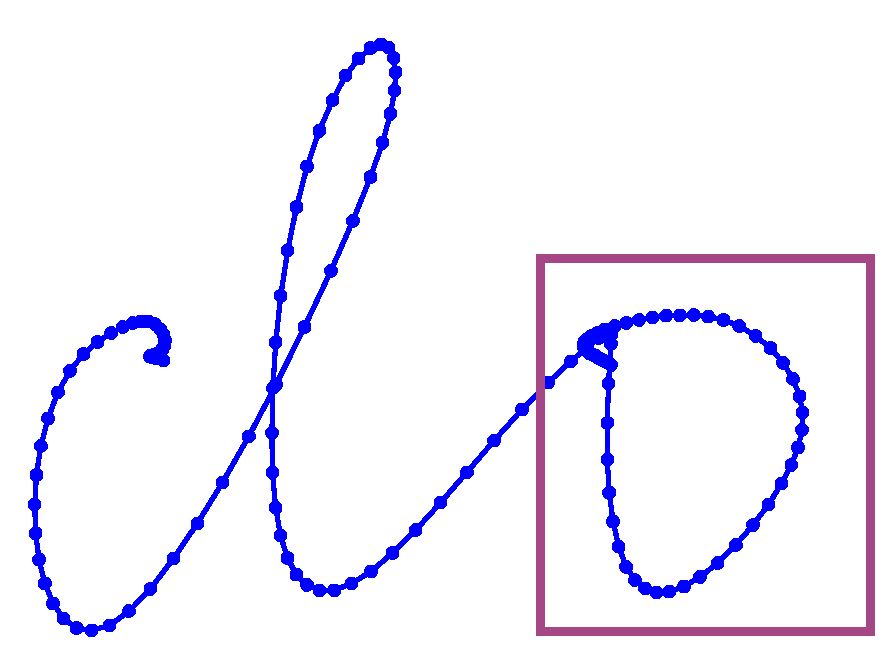
\includegraphics[width=0.09\columnwidth]{./Graphic/words_jing/1007_pdfCopy.eps}}
& 
{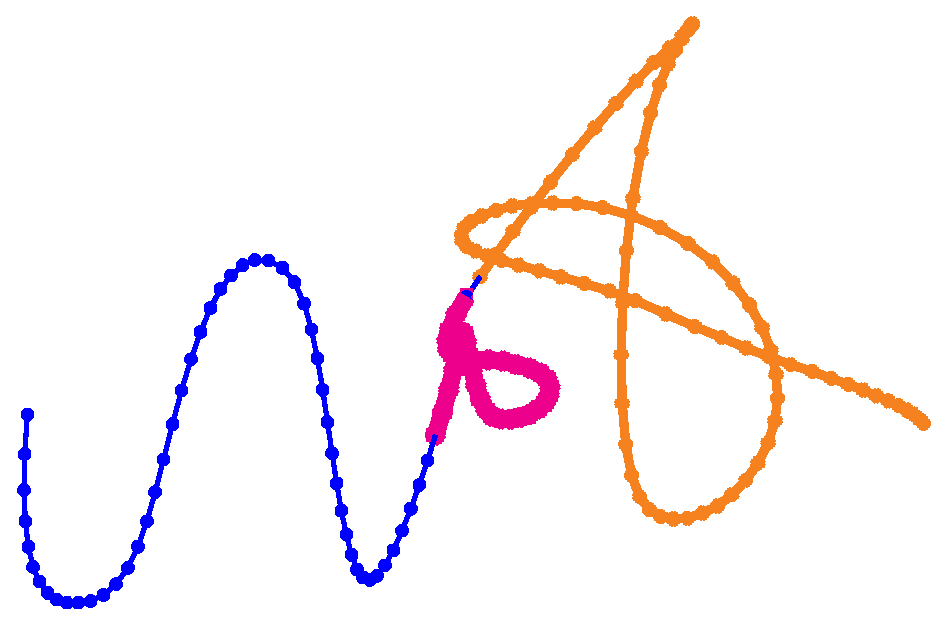
\includegraphics[width=0.09\columnwidth]{./Graphic/words_jing/1008_pdfCopy.eps}}
& 
{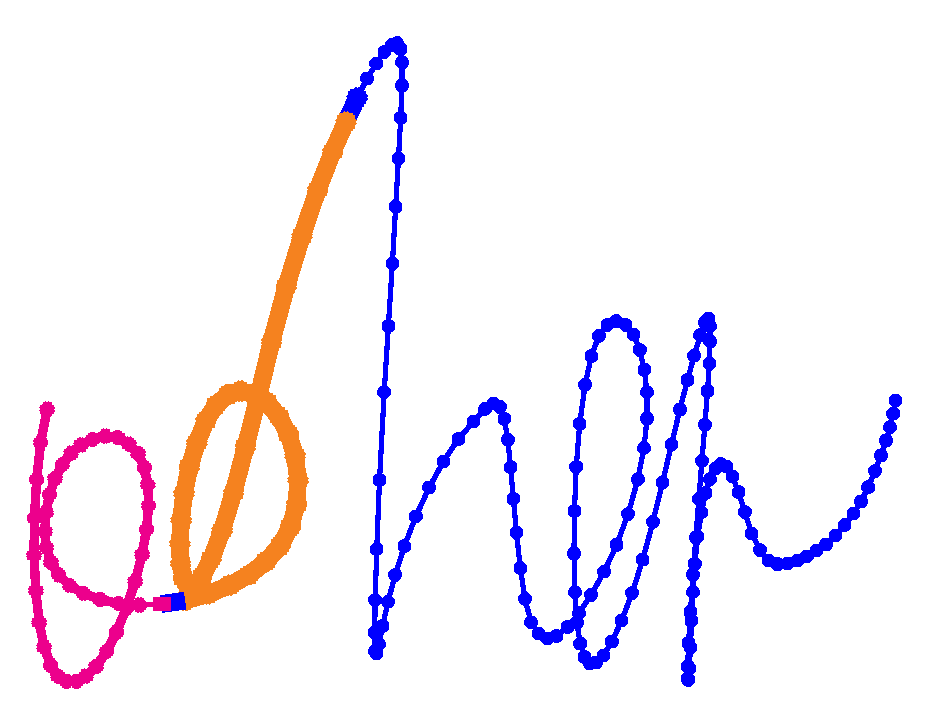
\includegraphics[width=0.09\columnwidth]{./Graphic/words_jing/1011_pdfCopy.eps}}
& 
{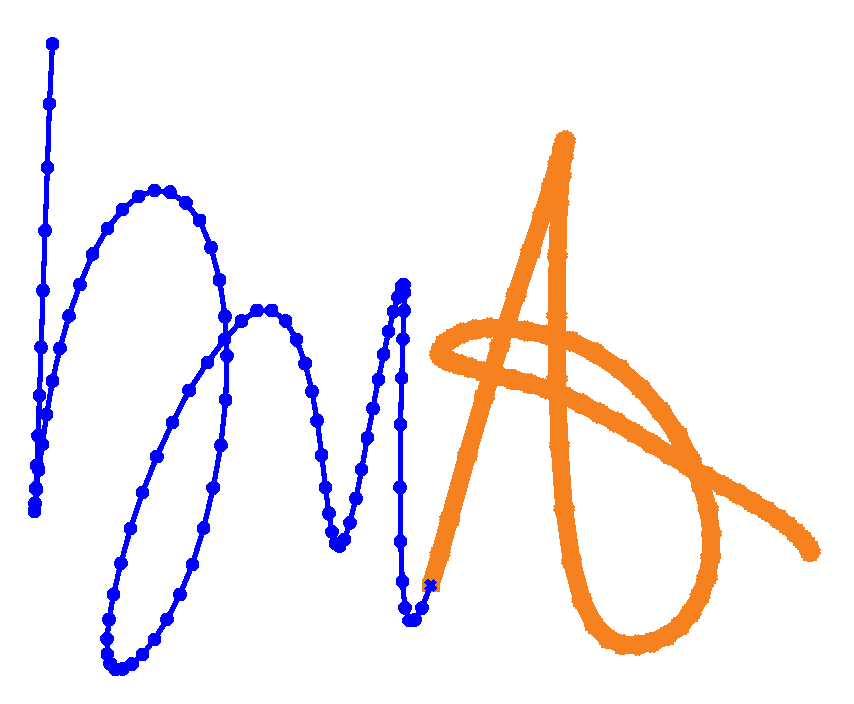
\includegraphics[width=0.09\columnwidth]{./Graphic/words_jing/1014_pdfCopy.eps}}
\\ 

 & \texttt{when} %& \texttt{it} 
 & \texttt{comes} & \texttt{out}  & \texttt{other} & \texttt{but} \\ 
\hline 
%\vspace{3mm}
User-2
& 
{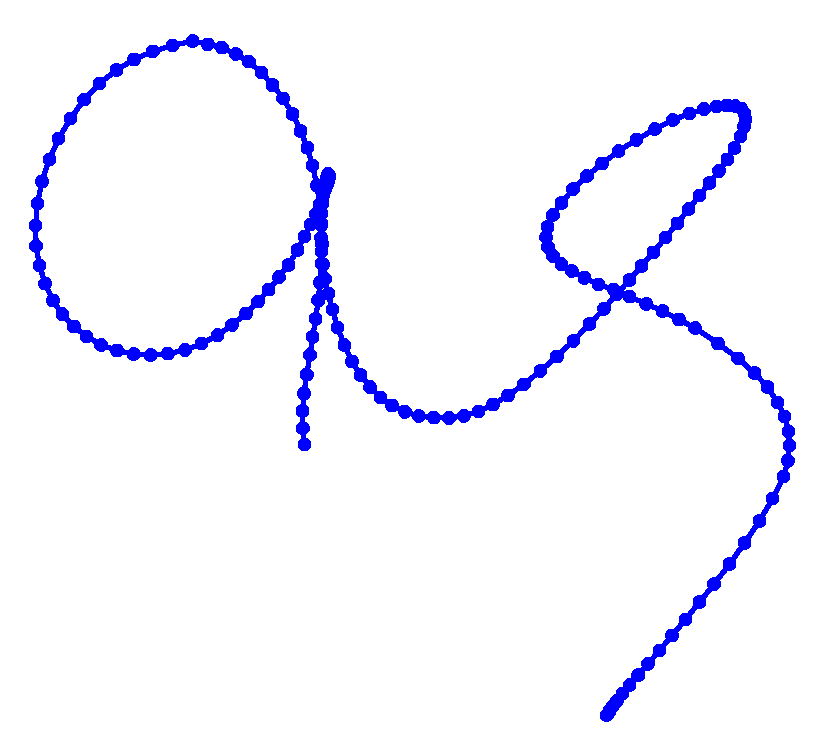
\includegraphics[width=0.09\columnwidth]{./Graphic/words_meng/10023_pdf.eps}}
%&
%{
\includegraphics[width=0.09\columnwidth]{./Graphic/words_meng/10026_pdf.eps}}
& 
{
\includegraphics[width=0.09\columnwidth]{./Graphic/words_meng/10030_pdf.eps}}
%& 
%{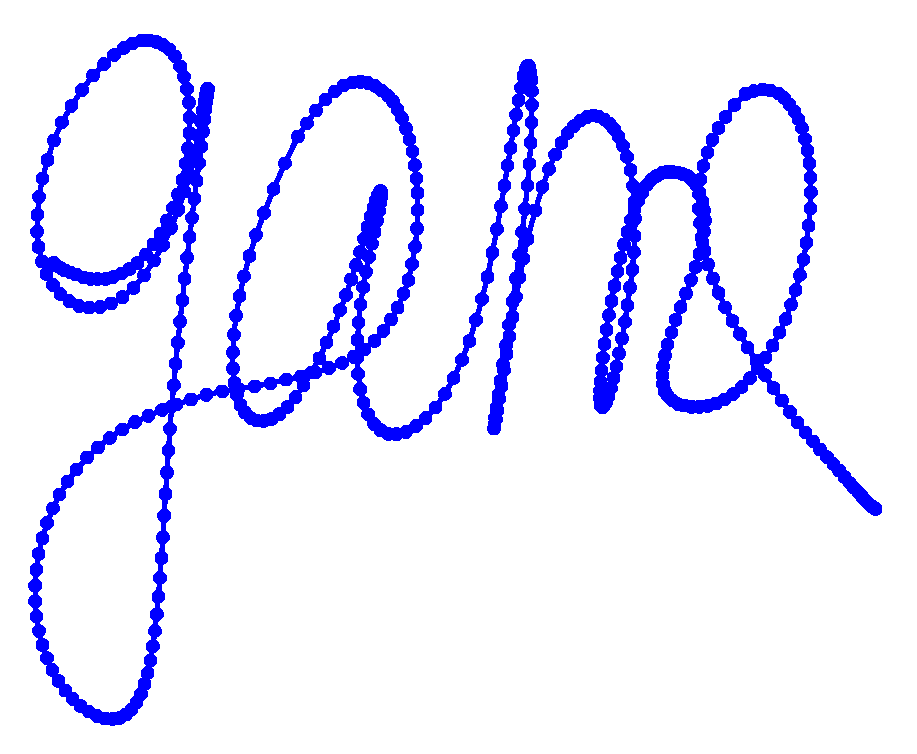
\includegraphics[width=0.09\columnwidth]{./Graphic/words_meng/20003_pdf.eps}}
%& 
%{
\includegraphics[width=0.09\columnwidth]{./Graphic/words_meng/20014_pdf.eps}}
%& 
%{
\includegraphics[width=0.09\columnwidth]{./Graphic/words_meng/20018_pdf.eps}}
& 
{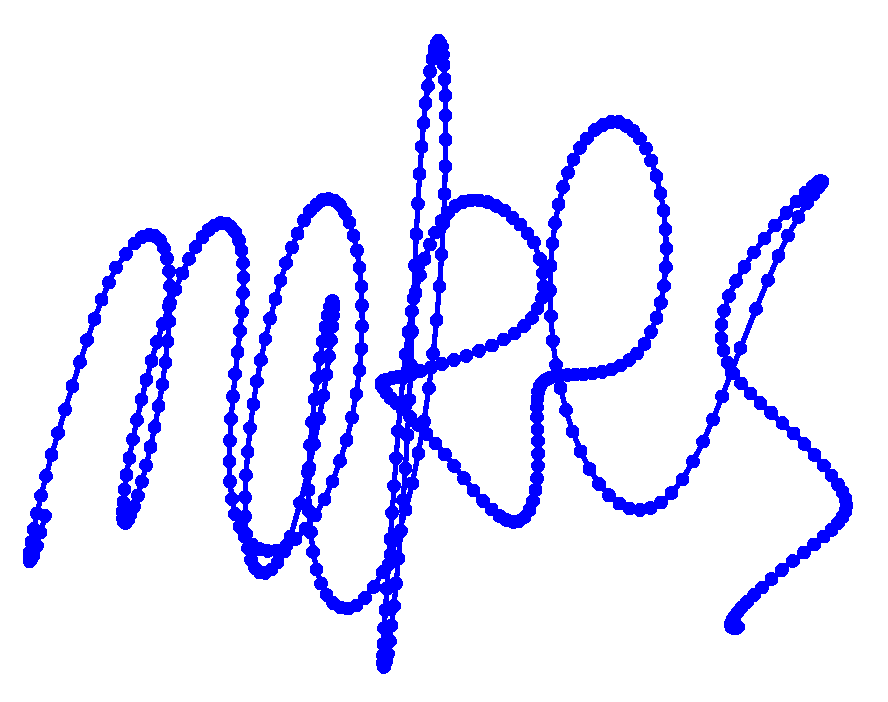
\includegraphics[width=0.09\columnwidth]{./Graphic/words_meng/20019_pdf.eps}}
& 
{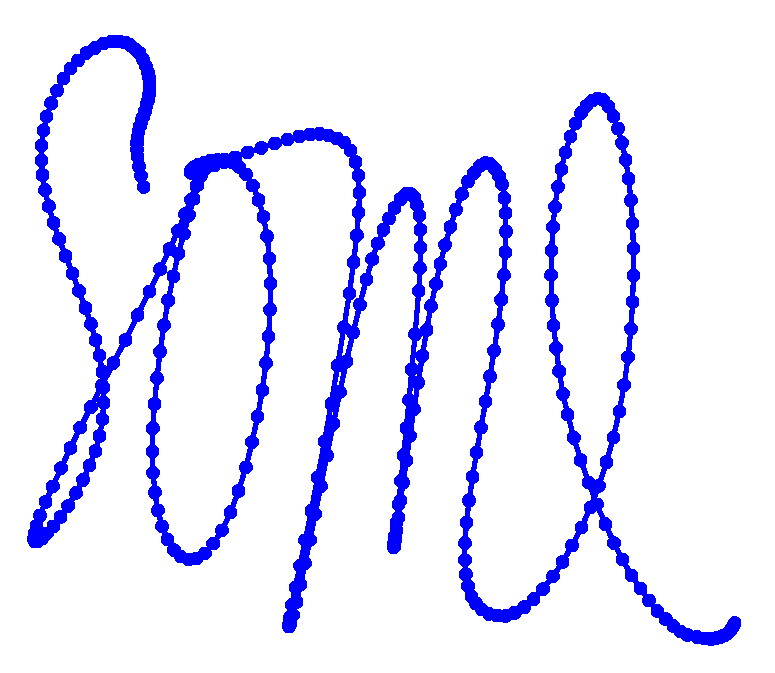
\includegraphics[width=0.09\columnwidth]{./Graphic/words_meng/20028_pdf.eps}}
& 
{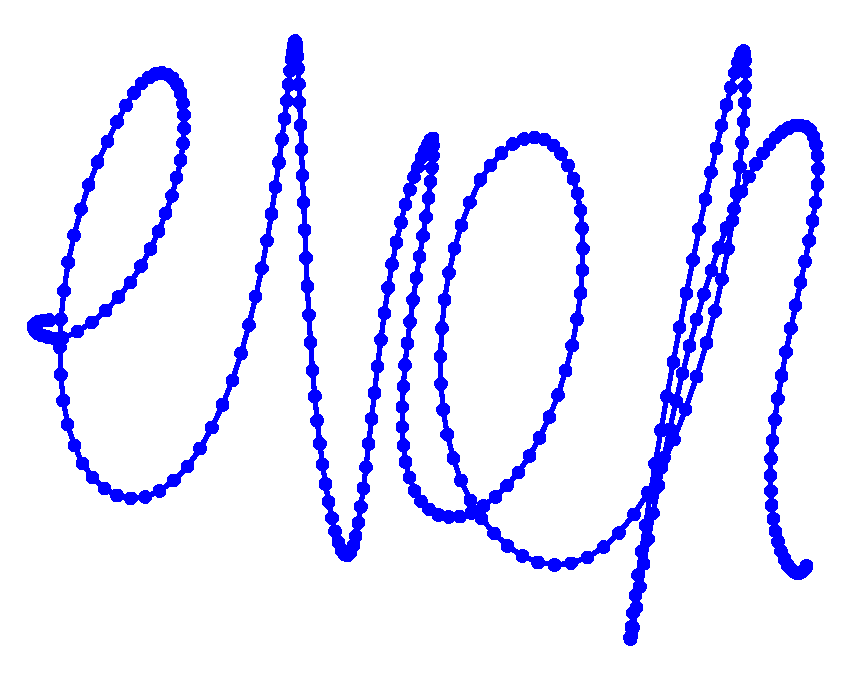
\includegraphics[width=0.09\columnwidth]{./Graphic/words_meng/20033_pdf.eps}}
\\ 
 & \texttt{as} %& \texttt{or} 
 & \texttt{with} & \texttt{makes}  & \texttt{some} & \texttt{even} \\ 
\hline
User-3
& 
{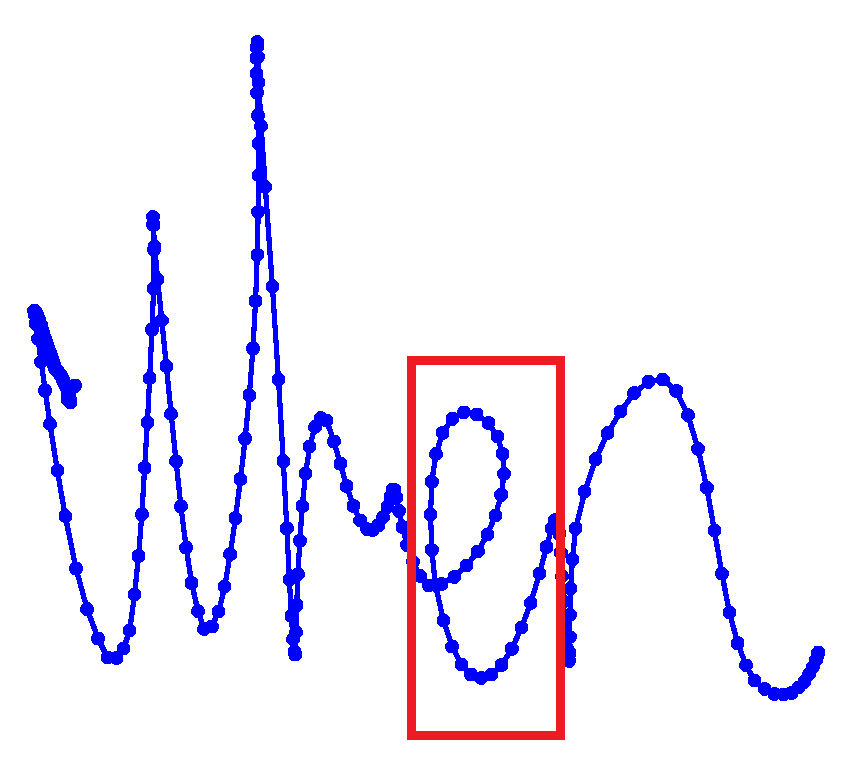
\includegraphics[width=0.09\columnwidth]{./Graphic/words_cao/10001_pdfCopy.eps}}
%&
%{
\includegraphics[width=0.09\columnwidth]{./Graphic/words_cao/10002_pdf.eps}}
& 
{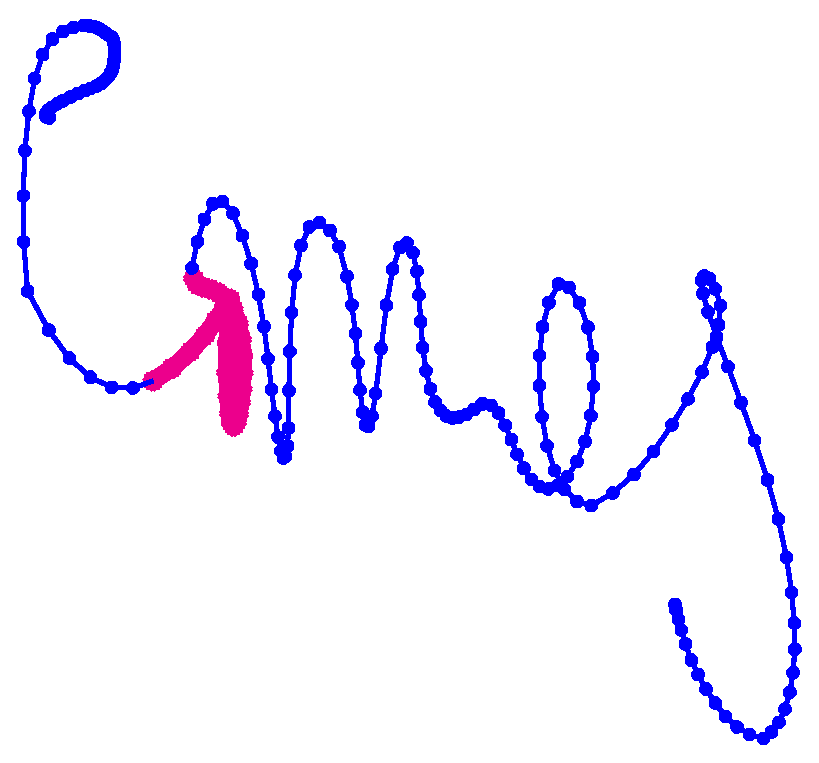
\includegraphics[width=0.09\columnwidth]{./Graphic/words_cao/10003_pdfCopy.eps}}
%& 
%{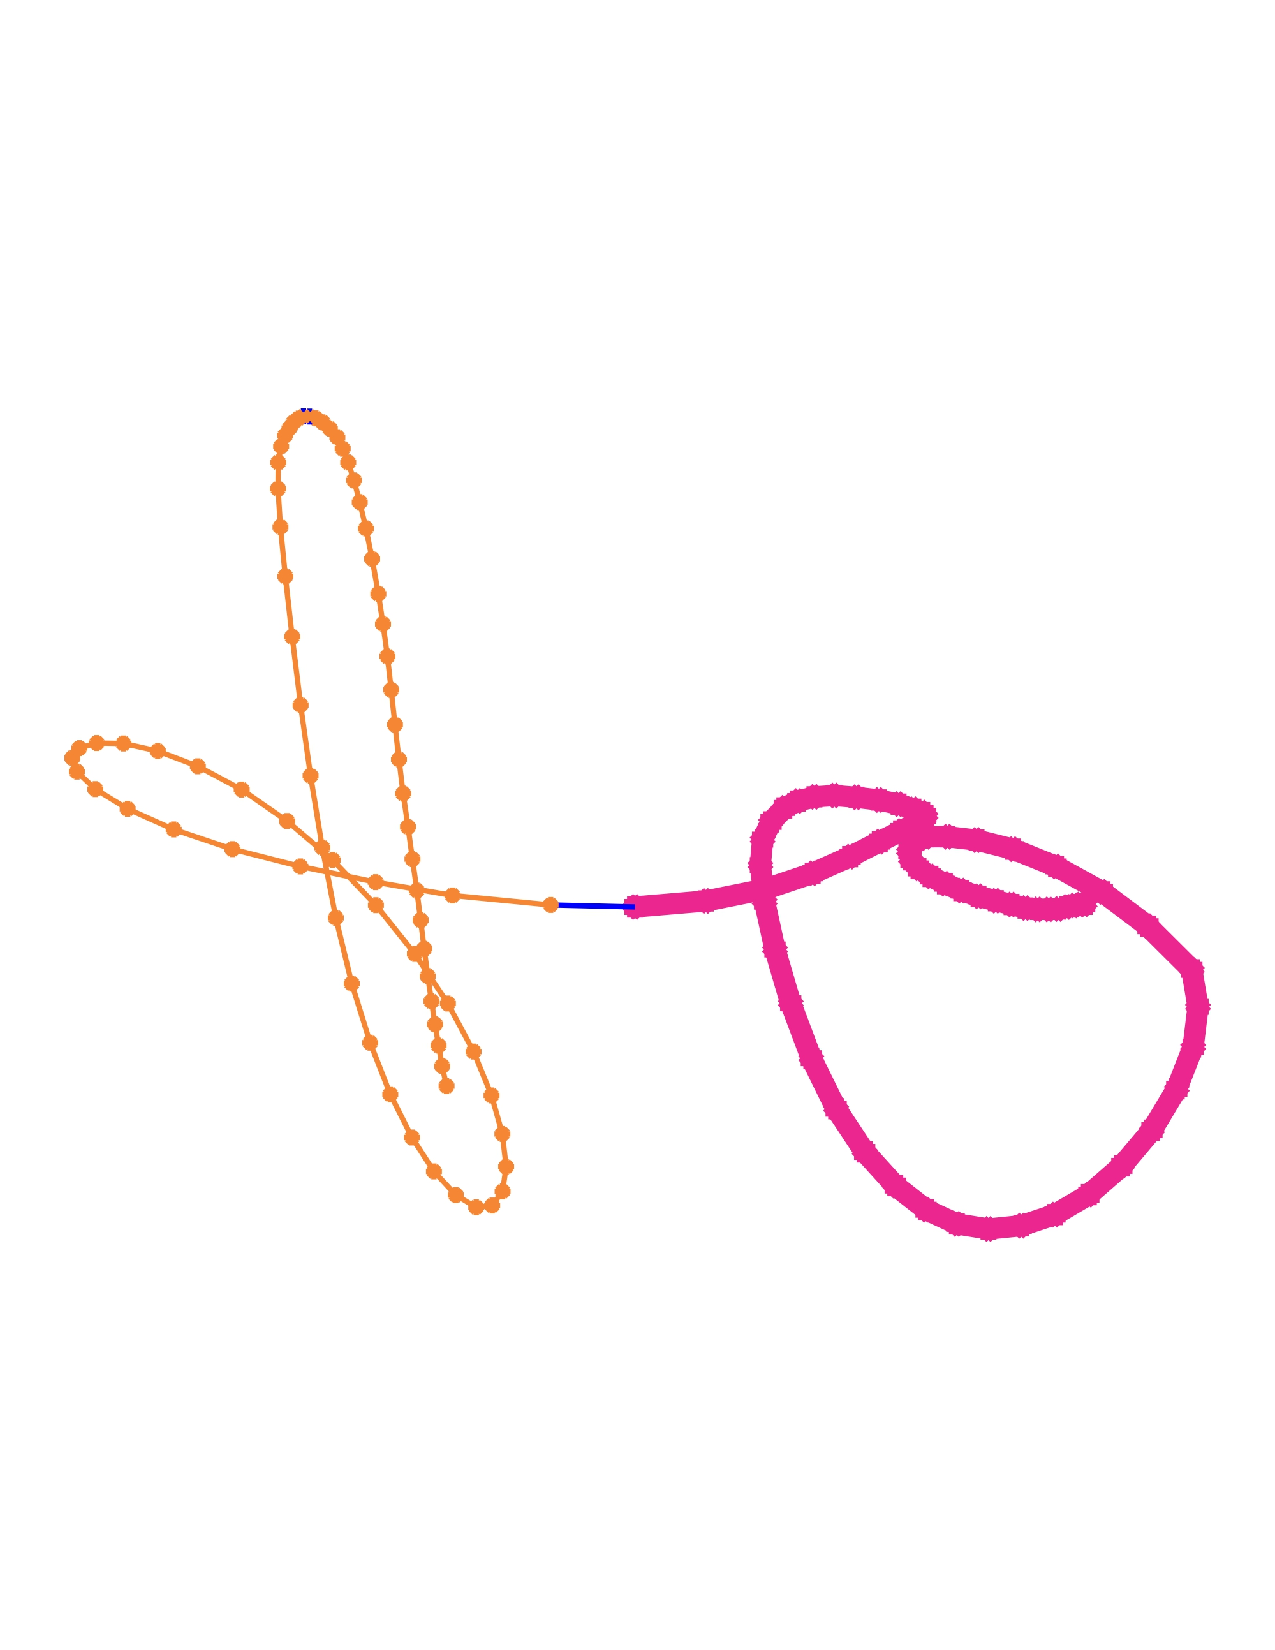
\includegraphics[width=0.09\columnwidth]{./Graphic/words_cao/10004_pdfCopy.pdf}}
%& 
%{
\includegraphics[width=0.09\columnwidth]{./Graphic/words_cao/10005_pdf.eps}}
%& 
%{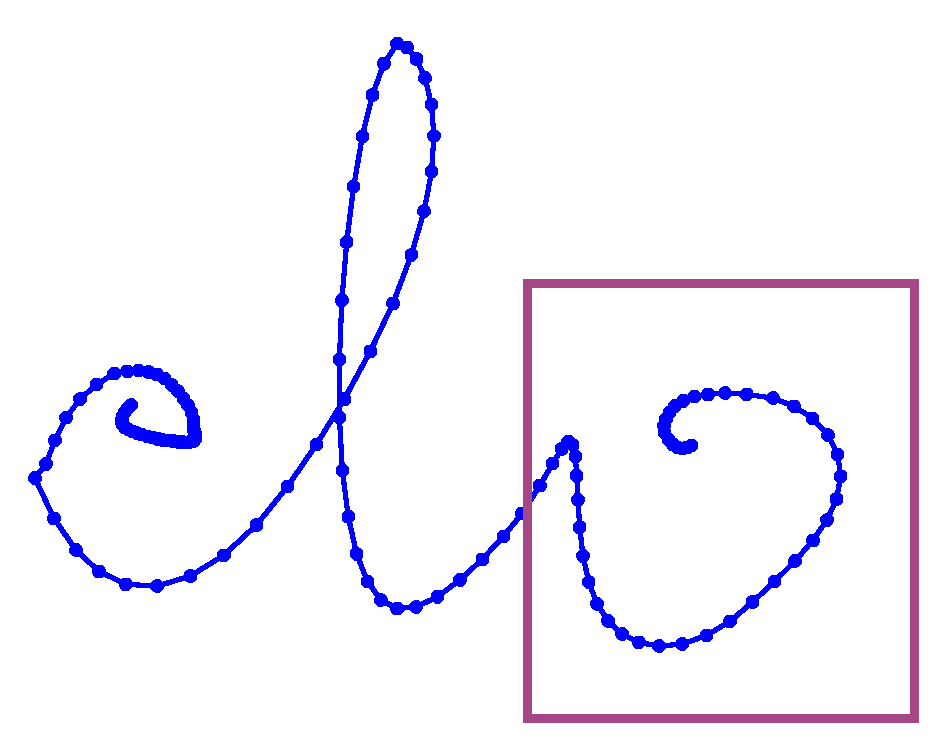
\includegraphics[width=0.09\columnwidth]{./Graphic/words_cao/10007_pdfCopy.eps}}
& 
{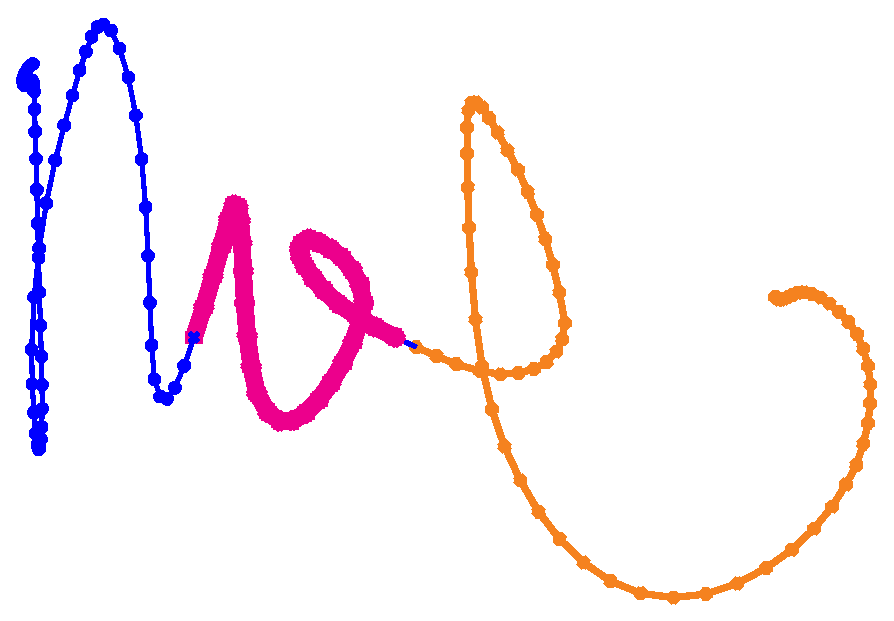
\includegraphics[width=0.09\columnwidth]{./Graphic/words_cao/10008_pdfCopy.eps}}
& 
{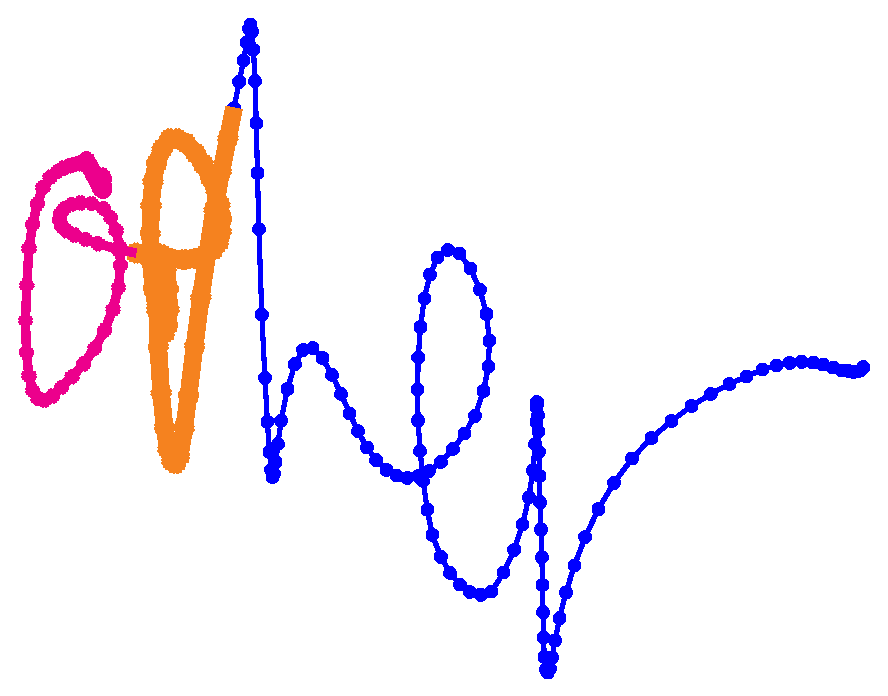
\includegraphics[width=0.09\columnwidth]{./Graphic/words_cao/10011_pdfCopy.eps}}
& 
{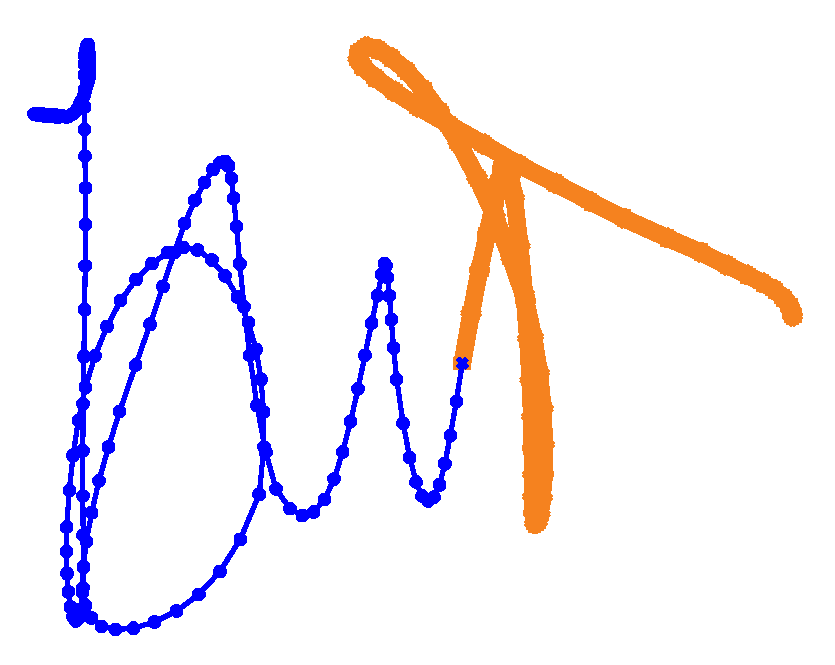
\includegraphics[width=0.09\columnwidth]{./Graphic/words_cao/10014_pdfCopy.eps}} 
\\ 
 & \texttt{when} %& \texttt{it} 
 & \texttt{comes} & \texttt{out}  & \texttt{other} & \texttt{but} \\ 
\hline
\end{tabular}
%\vspace{3mm}
\caption{\jing{Examples of processed trajectories written by two users. 
Despite that some handwritten words from User-1 and User-3 appear to be similar (e.g., \texttt{but}) yet some letters written by the same user may differ (e.g., the highlighted letters `o' and `t'), our authentication system can reliably distinguish them regardless of what they wrote. This is because \CiT is independent of text contents since it utilizes features derived at the scale of a stroke segment, e.g., \jingjuly{a short length of handwritten trajectory}.  
}\vspace{-3mm}}\label{fig:dataWords3user}

\end{figure}


%To track the motion of human fingers, we utilize depth sensors, because they are capable of capturing 3D human motion in a \textit{touch free} manner, just like how a camera captures pictures. Unlike behavior biometrics that rely on \textit{contact-based} input devices, such as touch screens~\cite{Kubota:ISPACS06,Liu:2009MobiHCI}, mouse movements~\cite{Zheng:CCS11,Ahmed:TPDS07}, keystroke dynamics~\cite{Monrose:CCS99,Revett:springerlink:10},  depth sensors eliminate hygiene concerns and smudge attacks~\cite{Aviv:woot10}.  Without loss of generality, we focus on utilizing a promising depth sensor --- a Leap Motion controller (in short, Leap Motion), which is designed to let users interact with a computer by waving their hands and fingers~\cite{LeapOnline1}, as shown in Figure~\ref{fig:leap}. Leap Motion captures the 3D motion of fingers at a relatively high precision 
%and tracks the finger length as well as width. This allows capturing behavior biometrics at a higher degree of freedom (i.e., entropy) than the traditional handwriting captured on flat surfaces (e.g., paper). 





%i.e., finger smudges (due to oily residues) on a touch screen can reveal passwords. In addition, unlike fingerprints, which are unsuitable to users with dirty, greasy, or worn-out fingerprints due to their professions (e.g., miners).


  

%Most of such biometrics is embedded in the usage pattern of various touch-based input devices, such as finger gestures when operating touch screens~\cite{Kubota:ISPACS06,Liu:2009MobiHCI}, mouse movements~\cite{Zheng:CCS11,Ahmed:TPDS07}, keystroke dynamics~\cite{Monrose:CCS99,Revett:springerlink:10}, etc. However, the recent advances in depth sensors has remarkably changed and will continue to alter the landscape of human-computer interaction. The trend urges us to explore new authentication schemes utilizing biometrics that is naturally built in the usage of the emerging depth sensors.

%, new input technologies, we explore new biometrics that can satisfy the re-authentication requirements that traditional text password and token-based authentication cannot offer.

%The emerge of low-cost depth sensors has remarkably changed and will continue to change the landscape of human-computer interaction, which was dominated by contact-based input devices, i.e., keyboards, mics, or touch screens. 
%Unlike contact-based input devices (i.e., touch screens~\cite{Kubota:ISPACS06,Liu:2009MobiHCI}, mouse movements~\cite{Zheng:CCS11,Ahmed:TPDS07}, keystroke dynamics~\cite{Monrose:CCS99,Revett:springerlink:10}), depth sensors are capable of capturing 3D human motion in a touch free manner, just like how a camera captures pictures. We have already witness how Microsoft Kinect~\cite{Kinect} and Leap Motion controller~\cite{LeapOnlineOverview} opened a new page for gaming and new apps. Looking forward, given that depth sensors enable a far less constrained input modalities than prior devices, they will become a non-dispensable part of future devices: Intel has announced to integrate RealSense 3D Cameras into mainstream computing devices~\cite{Intel}; Google has its plan of adding depth sensors into smartphones~\cite{Google}. In summary, the future human-computer interfaces are likely to be based on human motion, which simultaneously provides an opportunity for novel authentication schemes. 



%We design a new CS authentication scheme that is called \CiT, and the basic idea is to extract biometrics (also called \CiT) from finger movements when the user is writing in the air. When authenticate a user, the system randomly prompt a string on the screen as a challenge, and later the user write the string in the air as a response. The system authentication after receiving the response has two steps. First, recognize the handwriting to check if the content is the same as the challenge. Second, verify if the handwriting style is from a given user or from a given group of users. The handwriting recognition has been done by Tappert etc~\cite{Tappert1990}, thus our research focuses on the second part.



%To track the motion of human fingers as he/she writes in the air, without loss of generality, we focus on utilizing an emerging popular input device --- a Leap Motion controller (in short, Leap Motion), which is designed to let users interact with a computer by waving their hands and fingers~\cite{LeapOnline1}, as shown in Figure~\ref{fig:leap}.  


%Using depth sensors is advantageous: First, it captures the 3D motion of fingers %at a relatively high precision 
%and tracks the finger length as well as width. This allows capturing behavior biometrics at a higher degree of freedom (i.e., entropy) than the traditional handwriting captured on flat surfaces (e.g, paper). Second, operating in a contactless manner, it eliminates hygiene concerns and smudge attacks~\cite{Aviv:woot10}, i.e., finger smudges (due to oily residues) on a touch screen can reveal passwords. 
%Third, it is complementary to many traditional biometrics. For instance,   fingerprints have limitation and are inapplicable in several scenarios, e.g., fingerprints are unsuitable to users with dirty, greasy, or worn-out fingerprints due to their professions (e.g., miners).
%Forth, given the rich combination of letters and numbers, the continuously-written words are challenging to synthesize because imitating arbitrary handwriting in the 3 dimensional (3D)-space is ambitious. Thus, it is likely to be resistant to shoulder surfing. 
%Finally, writing words in the air might not be a completely natural way for entering information yet, but we optimistically predict that  users might adapt to it over time, similar to how users became familiar with keyboards. 




%We envision that \CiT can be used to authenticate users in a scenario insider attacker should be avoided. After initial user authentication, a user will receive a random string from the computer and interact with computers by writing towards a leap motion.
%%, since writing math symbols or formulas is preferable over typing. 
%Throughout the session, \CiT can harvest behavioral biometrics that is embedded in writing regardless of the writing content, so that it can verify users 
%% (i.e., identify a legitimate user out of a set of known candidates) 
%and raise an alarm when an alien is detected (i.e., an attacker tries to impersonate known candidates). 

%, who may share or have their individual motion depth sensors, enter comments by     some users may share the same input devices and enter comments by writing instead of typing, since writing math symbols or formulas is preferable over typing. In this case, it is promising to correctly exclude all aliens and identify each user regardless of what he/she writes, and inform the remote parties in real time. In summary, the goal is to perform re-authentication and have a high rejection rate for aliens and a high identification accuracy to determine user identity.% with a short delay.  



\CiT has to be \textit{content-independent} for CR authentication, because the CR authentication can require a user to write any content including letters, digits, and special symbols.
We design the second step of \CiT to rely on the handwriting style, i.e., authenticating based on `how you write' instead of `what you write'.   Building such an authentication system is challenging. First, extracting a  handwriting style from 3D movements captured by Leap Motion 
is non-trivial because of the overlapped finger trajectories created when a user is forced to write multiple words within a limited operation range of Leap Motion (i.e., approximately 25 to 600 mm above the device~\cite{LeapOnlineOverview}). In addition,  \CiT has to be reliable despite the handwriting variation of the same user (especially writing different content) and possible handwriting similarity between different users (especially writing the same content), and \CiT has to reject attackers.
\jing{ 
To characterize handwriting styles, we introduce the concept of \textit{stroke segment}: a segment of fingertip trajectory that is small enough to serve as writing style element.}


To make the classification computationally reasonable and better represent the writing style, we propose a transition co-occurrence matrix. %Generating features out of components directly leads to a high-dimension feature vector, which make the classification extremely computationally heavy. Thus, we use feature reduction techniques  and propose a transition co-occurrence matrix for easy classification. 
%Each point of a writing component has several kinematic features. To reduce the feature dimensions of a writing component, we use a $K$-means clustering method to find typical writing components and design the final feature as a component transition co-occurrence matrix. 
\jing{We use a \textit{sample}, i.e.,  a piece of handwriting (e.g., a trajectory recorded in 5 seconds,) to represent a user’s handwriting style.} By combining co-occurrence matrices extracted from data samples and an effective classification method --- Support Vector Machine (SVM), we are able to authenticate users reliably.  For example,  \figref{fig:dataWords3user} illustrates handwriting of two users. Despite that some handwritten words by User-1 and User-3 appear to be similar (e.g., \texttt{but}) yet some letters written by the same user may differ (e.g., the highlighted letters `o' and `t'), our authentication system can reliably distinguish them regardless of what they wrote. This is because \CiT is designed to be independent of text contents and utilizes features derived at the scale of a writing stroke segment.
Encouragingly, our system can correctly identify all the three users, despite the visual similarity between handwritten words with the same content written by User-1 and User-3. %\jing{While, the authentication methods based on content comparing, e.g., dynamic time warping used in~\cite{TianQXW13:NDSS13},  cannot complete such a task.}
%
%Second, if an attacker tries to imitate a legitimate user, \CiT has to be able to detect it as an alien.
%
The main contributions of this paper are listed below. 
\begin{itemize}
\vspace{-1.5mm}
%\setlength{\itemsep}{-1mm}
\item We designed a motion-based challenge-response authentication that we call \CiT. \CiT models handwriting styles in the 3D space and can authenticate users independent on what they write, e.g., English letters, math symbols, diagrams, or digits. 

\item We proposed a novel 3-level feature extraction method that derives a co-occurrence matrix. Thus we reduce the feature dimension, keep temporal information and statistically represent writing styles. 

\item We built a system that uses the latest motion sensor, a Leap Motion controller, to capture users' writing movements in the air and performed classification using SVM. 


\item We evaluated \CiT on 24 subjects over 7 months and 7 observing attackers.
The CR authentication results show that the average equal error rate is 1.18\% for random insider attacks and 2.45\% for random impostors when testing with 17.5 seconds of handwriting. Besides, we could achieve an average error rate of 3.11\% testing with 8.8 seconds of handwriting. In addition, \CiT can reliably reject observing attackers.

\vspace{-1mm}
\end{itemize}

We organize the remainder of the paper as follows. \jing{We define the attack model, discuss the background of Leap Motion and related work in~\secref{sec:background}. In~\secref{sec:overview}, we discuss the feasibility of authenticating a user using 3D handwriting styles, and show an overview of the \CiT system.} Then, we present the data processing in~\secref{sec:data}, and feature extraction schemes as well as a classification method in~\secref{sec:feature} and show results in\secref{sec:results}. Finally, \jing{we present some discussion and conclude in \secref{sec:conc}}. 

